\documentclass[11pt, a4paper]{article}

%\usepackage[T1]{fontenc}
%\usepackage{fullpage}

\usepackage[utf8]{inputenc} % comment when using lualatex
\usepackage[italian]{babel} % lingua e a-capo-sillabato
\usepackage{graphicx}
\usepackage[hidelinks]{hyperref} % link di pagina
\usepackage[bottom]{footmisc} % note appiccicate al fondo della pagina
\usepackage{float} % per posizionamento immagini
\usepackage{amsthm} % per ambienti stile teorema
\usepackage{tabularx} %tabelle
\usepackage[table]{xcolor} %colore caselle
\usepackage{enumitem} %additional commands for lists
\usepackage{fancyhdr}
\usepackage[font=footnotesize,labelfont=bf]{caption} % small caption font-size



\pagestyle{fancy}
\fancyhf{}% Clear header/footer
\fancyfoot[C]{\thepage} %add page number
\fancyhead[C]{\footnotesize\textit{Documento:} D3 \hfill SleepCode \hfill \textit{Versione:} 1.0}
\renewcommand{\headrule}{{\color{red!70}\rule{\textwidth}{2pt}}}
\setlength{\headheight}{22pt}

\renewcommand\UrlFont{\color{blue}\rmfamily} % colore link

\theoremstyle{definition} % stile dei newtheorem (non italizzati)
\newtheorem{funcreq}{RF} %% numerazione dei requisiti funzionali
\newtheorem{nonfuncreq}{RNF} %% requisiti non funzionali
\newtheorem{backend}{BE}
\newtheorem{frontend}{FE}




\title{Documento di Architettura}

\author{Raffaele \textsc{Castagna}\\
Alberto \textsc{Rovesti}\\
Zeno \textsc{Saletti}}

\newcommand{\groupNumber}{G17}

% Web address for the project (if any)
% \newcommand{\homepage}{\url{https://www.}}

% data
\date{\today}

\makeatletter{}

\newcommand\blfootnote[1]{%
  \begingroup
  \renewcommand\thefootnote{}\footnote{#1}%
  \addtocounter{footnote}{-1}%
  \endgroup
}

% IL PREAMBOLO FINISCE QUI %%%%%%%%%%%%%%%%%%%%%%%%%%%%%%%%%%%%%%%%%%%%%%%%%%%%



\begin{document}

% La pagina di copertina si trova in un file .tex a parte
% NON MODIFICARE QUESTO COMANDO!!!
\begin{titlepage}
\newcommand{\HRule}{\rule{\linewidth}{0.3mm}} % Defines a new command for horizontal lines, change thickness here
\center % Centre everything on the page

%------------------------------------------------
%	Logo
%------------------------------------------------

\includegraphics[width=0.3\textwidth]{materiale/UniTrento_logo_ITA_colore.png}\\[0.5cm]
%------------------------------------------------
%	Headings
%------------------------------------------------
\textsc{\Large Dipartimento di Ingegneria\\e Scienza dell'Informazione}\\[1.5cm]

{\Huge\textbf{Sleep Code}}\\[0.5cm]
\textsc{\large Progetto per il Corso di Ingegneria del Software}\\
\textsc{\large Anno Accademico 2023-2024}\\[0.5cm]

%------------------------------------------------
%	Title
%------------------------------------------------

\HRule\\[0.4cm]
{\huge\bfseries \@title}\\[0.1cm]
\HRule\\[1cm]

\begin{minipage}{\textwidth}
\begin{flushleft}
\textit{Descrizione:} documento di analisi dei requisiti funzionali, non funzionali, front-end e back-end.
\end{flushleft}
\end{minipage}\\[1.5cm]


\begin{minipage}{0.4\textwidth}
\begin{flushleft}
\large
\textit{Numero documento:} D1
\end{flushleft}
\end{minipage}
\begin{minipage}{0.4\textwidth}
\begin{flushright}
\large
\textit{Versione documento:} 2.4
\end{flushright}
\end{minipage}\\[1.5cm]

%------------------------------------------------
%	Author(s)
%------------------------------------------------
\begin{minipage}{0.4\textwidth}
\begin{flushleft}
\large
\textit{Membri del gruppo:}\\
\@author % Your name
\end{flushleft}
\end{minipage}
~
\begin{minipage}{0.4\textwidth}
\begin{flushright}
\large
\textit{Numero gruppo: }
\groupNumber
\end{flushright}
\end{minipage}

% 	If you don't want a supervisor, uncomment the two lines below and comment the code above
% 	{\large\textit{Author(s)}}\\
% 	\@author % Your name

%------------------------------------------------
%	Date
%------------------------------------------------

\vfill\vfill
\textit{Ultima revisione:}
{\@date}

\end{titlepage}

\tableofcontents\blfootnote{\textbf{Consigli utili per la consultazione del testo:} Se il lettore per file \texttt{.pdf} attualmente in uso lo consente, è possible navigare con più semplicità e velocità all'interno di questo documento cliccando sugli elementi dell'indice.}

\newpage

\section*{Scopo del documento}
In questo documento viene riportata la definizione dell'architettura del
progetto \textit{SleepCode} impiegando diagrammi delle classi, realizzati
secondo gli standard di Unified Modeling Language (UML), e codice scritto in Object
Constraint Language (OCL). Nel documento precedente (D2, \textit{Specifica
dei Requisiti}) sono stati presentati il diagramma degli use case, quello
di contesto e infine il Diagramma dei Componenti. Considerando tale
progettazione, viene ora definita l'architettura del sistema specificando
in modo più dettagliato le classi implementabili sotto forma di
codice, insieme alla logica che regola il comportamento del software che
si intende realizzare.

Il linguaggio UML, utilizzato per descrivere le classi, è supportato da
codice OCL, impiegato invece per catturare gli aspetti logici citati sopra,
che non sarebbero altrimenti esprimibili formalmente mediante i soli diagrammi delle
classi.

Il diagramma finale, comprensivo di classi e codice OCL, è mostrato in
Figura \ref{umlocl} presente nell'ultima pagina di questo documento


\newpage
\section{Definizione delle classi}
Nella presente sezione vengono illustrate in linguaggio UML le classi
previste dal progetto \textit{SleepCode}. Ogni componente del diagramma
dei componenti, presente nel documento D2, viene qui rappresentato
in forma di una o più classi.

%Le classi individuate sono costituite
%da un nome, un insieme di attributi che identificano i dati gestiti dalla
%classe stessa e una lista di metodi che definiscono le operazioni
%eseguibili da quella classe. Eventuali relazioni tra classi sono evidenziate
%da alcune associazioni.

\subsection{Utenti}
L'attore che nel diagramma di contesto usufruisce delle funzionalità offerte
dal sistema è l'utente. Come descritto nei documenti di Analisi (D1) e
e Specifica dei Requisiti (D2), esistono tre categorie di utenti: anonimo, autenticato
e amministratore. La Figura \ref{utenti} illustra le rispettive classi.

\begin{figure}[H]
\centering
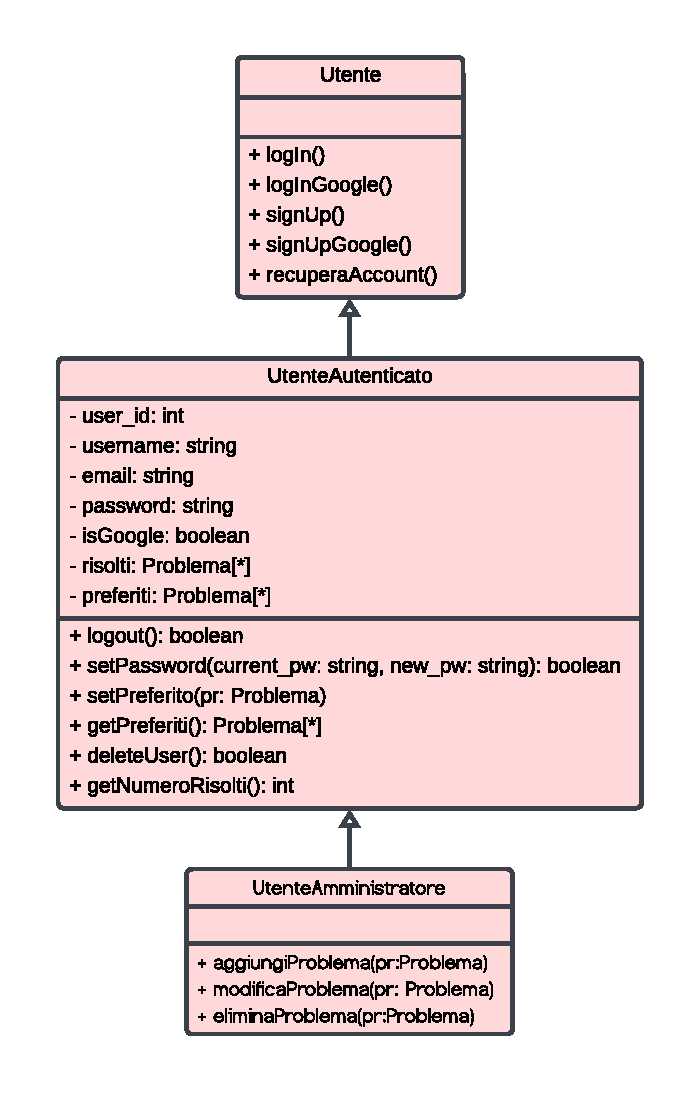
\includegraphics[scale = 0.65]{materiale/class-utenti.pdf}
\caption{Definizione della classe \texttt{Utente} e delle sue sottoclassi}
\label{utenti}
\end{figure}

Dal momento che tutte queste categorie condividono alcune funzionalità, è stata
creata una classe \texttt{Utente}, che logicamente corrisponde alla categoria
degli utenti anonimi, ovvero utenti che non hanno effettuato il login. Di fatto,
non è prevista la memorizzazione di alcuna informazione riguardo a questa categoria
di utenti e le operazioni disponibili sono:
\begin{itemize}
    \item \texttt{login}: richiesta di accesso con sistema di credenziali interne.
    \item \texttt{signUp}: richiesta di registrazione con sistema di credenziali interne.
    \item \texttt{loginGoogle, signUpGoogle}: controparti dei metodi precedenti, che
    però si avvalgono dei servizi di autenticazione Google.

    \item \texttt{recuperaAccount}: richiesta di avvio della procedura di recupero account.
\end{itemize}
Da questa prima classe viene definita, mediante generalizzazione, la classe
\texttt{UtenteAutenticato}, che aggiunge metodi e attributi accessibili previo
login:
\begin{itemize}
    \item \texttt{user\_id}: questo attributo riveste il ruolo di identificatore
    univoco dell'account dell'utente registrato ed eventualmente autenticato.

    \item \texttt{username, email, password}: i dati richiesti per creare un
    account. In caso di autenticazione con Google, è richiesto che la classe
    memorizzi solo l'indirizzo email impiegato e l'username.

    \item \texttt{isGoogle}: parametro che distingue gli account collegati con
    Google da account registrati con il meccanismo di credenziali interne.

    \item \texttt{risolti, preferiti}: insiemi dei problemi, rispettivamente,
    risolti dall'utente e salvati come preferiti dall'utente.

    \item \texttt{logout}: richiesta di logout.
    
    \item \texttt{setPassword}: procedura atta a modificare la password
    dell'account. Oltre alla nuova password, viene richiesta, per ragioni di
    sicurezza, la password attualmente in uso. Viene restituita una risposta
    di tipo booleana per segnalare il successo o l'insuccesso dell'operazione.

    \item \texttt{setPreferito}: questo metodo provvede ad aggiungere o
    eliminare dalla lista dei preferiti dell'utente il problema fornito: se
    presente, esso viene rimosso dalla lista, altrimenti viene aggiunto
    (viene inoltre incrementato il valore dell'attributo \texttt{preferito}
    della classe \texttt{Problema}, descritta nelle prossime sezioni).

    \item \texttt{getPreferiti}: i preferiti dell'utente autenticato vengono
    messi a diposizione all'esterno della classe grazie a questo metodo.
    Come descritto nel diagramma dei componenti, in questo modo viene
    realizzata l'interfaccia che passa i preferiti dell'utente dal Gestore
    Utente verso il Catalogo, in modo da visualizzarli nella lista dei
    problemi.

    \item \texttt{deleteUser}: il metodo per l'eliminazione dell'account
    restituisce un valore booleano per notificare l'esito dell'operazione.

    \item \texttt{getNumeroRisolti}: il valore restituito rappresenta i
    progressi dell'utente, ovvero il numero di problemi risolti rispetto
    al totale presente nel catalogo. Questo valore viene calcolato in base
    al numero di problemi presenti in \texttt{risolti} e attualmente
    memorizzati nel database.
\end{itemize}
Infine, un'ulteriore generalizzazione specifica le funzionalità aggiuntive
dell'utente amministratore, ovvero metodi utili alla gestione del catalogo
e dei problemi:
\texttt{aggiungiProblema}, \texttt{modificaProblema}, \texttt{eliminaProblema}.


Facendo riferimento al Diagramma dei Componenti del
documento D2, queste classi sono state estratte da tre componenti
distinti che si occupano dell'interazione con l'utente esterno: dalla
\textit{Pagina di Autenticazione} sono stati raggruppate le interfacce che
si trovano in \texttt{Utente}; nella classe \texttt{UtenteAutenticato} sono state
raccolte le interfacce presenti nel componente \textit{Gestore Profilo};
in \texttt{UtenteAmministratore} sono state raggruppate le interfacce
definite nel componente \textit{Catalogo}.


\subsection{Gestione autenticazione}
Nel diagramma di contesto, l'autenticazione si avvale di due sistemi
subordinati: \textit{Firebase}, che si occupa di memorizzare gli account
registrati con sistema di autenticazione interno, e \textit{Google SignIn},
con il quale è possibile effettuare la registrazione o l'autenticazione
mediante un account Google.

Il componente \textit{Gestore Autenticazione} del rispettivo diagramma si
occupa di interagire con tali sistemi esterni in modo da convalidare le
operazioni di registrazione e autenticazione. Per questo motivo, nel diagramma
delle classi viene individuata la classe \texttt{Autenticazione} (Figura \ref{autenticaz}):
\begin{itemize}
    \item \texttt{autorizzato}: questo attributo mantiene lo stato dell'autorizzazione
    dell'utente.

    \item \texttt{registraAccount}: questo metodo esegue la registrazione
    comunicando con il servizio di database.
    \item \texttt{autentica}: l'autenticazione mediante credenziali interne
    avviene grazie a questo metodo.
    \item \texttt{registraGoogle, autenticaGoogle}: analoghi ai precedenti,
    questi metodi si occupano delle operazioni di registrazine ed auteticazione
    con Google.
\end{itemize}
Tutti i metodi comunicano all'esterno l'esito delle loro operazioni mediante
un valore booleano di ritorno.

\begin{figure}[H]
\centering
%\hspace*{-1.9cm}
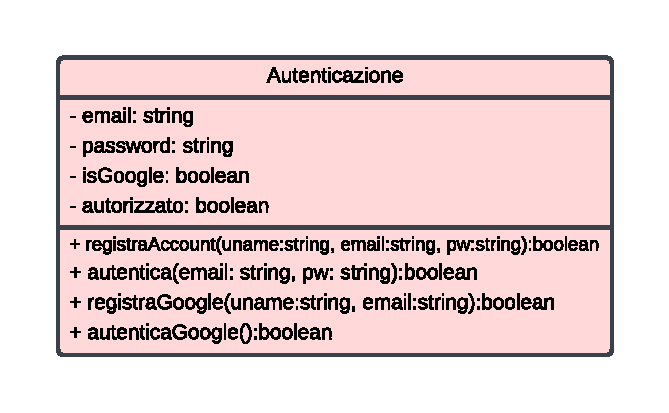
\includegraphics[scale = 1.1]{materiale/class-autenticazione.pdf}
\caption{Definnizione della classe \texttt{Autenticazione}}
\label{autenticaz}
\end{figure}


\subsection{Recupero della password}
Nel Diagramma dei Componenti viene individuata la \textit{Pagina di Recupero},
che offre supporto agli utenti registrati, con sistema di credenziali interne,
che hanno dimenticato la password e che intendono recuperare l'account.
Nel Diagramma di Contesto, il servizio di posta elettronica rientra nello
scambio di informazioni necessario per la procedura di recupero. Per
questi motivi viene definita la classe \texttt{RecuperoPwUtente} (Figura \ref{recupero}), che
raccoglie attributi e metodi necessari per effettuare il recupero,
interagendo tra l'altro con il servizio di posta elettronica.

\begin{itemize}
    \item \texttt{email}: l'indirizzo email di recupero viene memorizzato
    per conservarlo durante tutta la procedura di recupero.

    \item \texttt{inviaEmailRecupero}: il messaggio di recupero viene inviato
    all'indirizzo specificato. Questo metodo rappresenta la richieste di
    invio da parte del sistema nei confronti del servizio di posta.
\end{itemize}
Questa classe non si occupa dell'operazione di modifica effettiva della
password, a carico di Firebase. Essa interagisce solo con il servizio
di posta.

\begin{figure}[H]
\centering
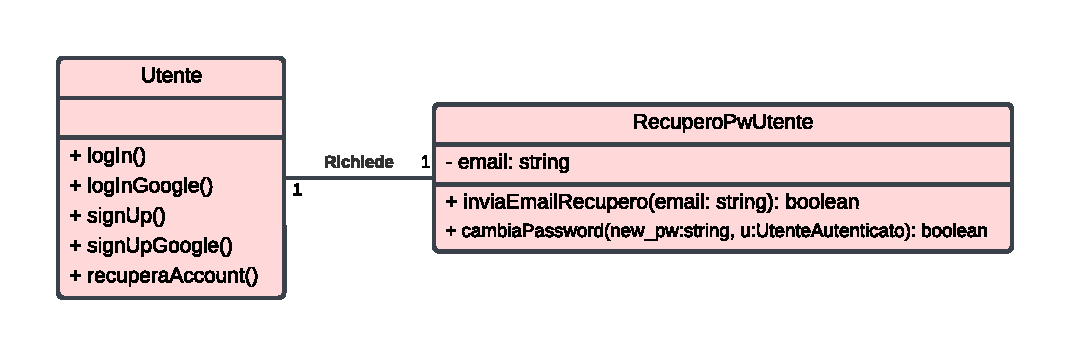
\includegraphics[scale = 0.85]{materiale/class-recupero.pdf}
\caption{Specifica architetturale del componente \textit{Pagina di Recupero} con la classe \texttt{RecuperoPwUtente}}
\label{recupero}
\end{figure}



\newpage
\subsection{Catalogo}
Il \textit{Catalogo} presente nel Diagramma dei Componenti è rappresentato in
Figura \ref{catalog} sotto forma di due classi principali: \texttt{UtenteAmministratore}, descritto insieme
alle altre categorie di utenti, e \texttt{Catalogo}. Tale scelta architetturale
è giustificata dall'esigenza di identificare chiaramente il ruolo dell'utente
amministratore, mantenendo dunque una definizione dei livelli di accesso
coerente con quella dei documenti precedenti, oltre alla volontà di ridurre il
carico di informazione della classe \texttt{Catalogo} rendendo il rispettivo
componente del diagramma più modulare e meno monolitico.

\begin{figure}[H]
\centering
\hspace*{-3cm}
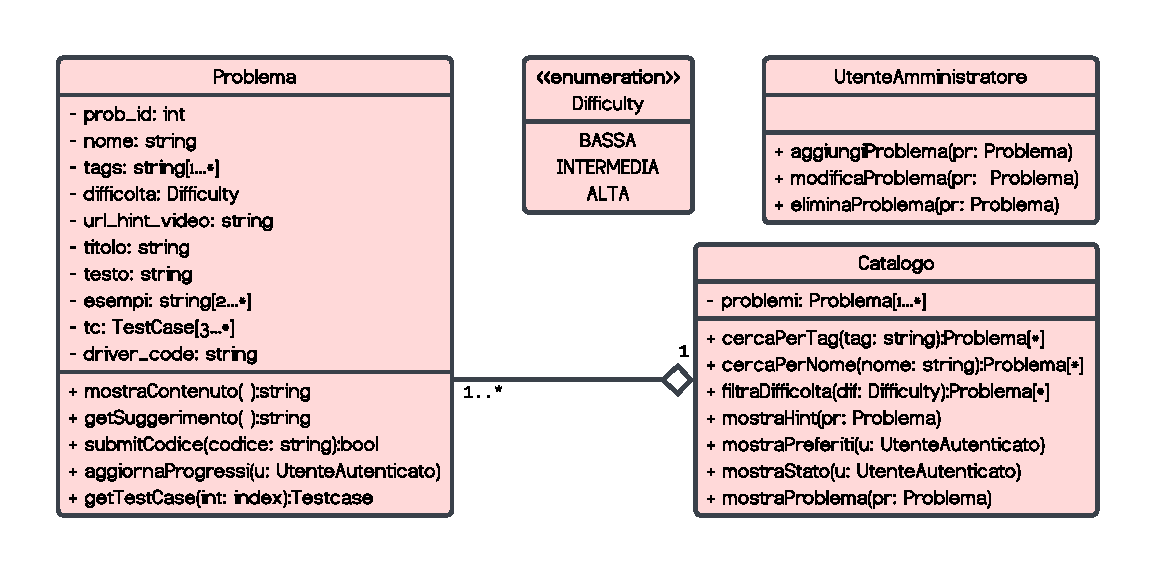
\includegraphics[scale = 0.9]{materiale/class-catalogo.pdf}
\caption{Specifica architetturale del componente \textit{Catalogo} con la classe \texttt{Catalogo}}
\label{catalog}
\end{figure}
\noindent La Figura \ref{catalog} mostra anche la classe \texttt{Problema},
descritta dettagliatamente nella prossima sezione. Il catalogo
raccoglie i problemi disponibili sulla piattaforma, quindi \texttt{Catalogo}
è legato a \texttt{Problema} da un'associazione di aggregazione.


\begin{itemize}
    \item \texttt{problemi[1...*]}: questo attributo indica che il catalogo
    consiste in una lista di almeno un problema.

    \item \texttt{mostraSuggerimento}: sulla base del metodo selezionato, il metodo
    interagisce con YouTube per richiedere la riproduzione del video-suggerimento.

    \item \texttt{mostraPreferiti}: sulla base dei dati dell'account
    dell'utente (autenticato), vengono contrassegnati i problemi preferiti
    all'interno del catalogo.

    \item \texttt{mostraStato}: come per il metodo precedente, il
    \texttt{Catalogo} mostra lo stato dei problemi, evidenziando quelli
    già risolti dall'utente autenticato.

    \item \texttt{mostraProblema}: questo metodo richiede l'apertura
    di un problema selezionato dall'utente, permettendo di consultare il
    contenuto e accedere alla rispettiva area di esercitazione.
\end{itemize}



\newpage
\subsection{Problemi ed Esercitazione}
La Figura \ref{esercitaz} illustra le classi che costituiscono il componente
\textit{Pagina di Esercitazione}.

\begin{figure}[H]
\centering
%\hspace*{-1.5cm}
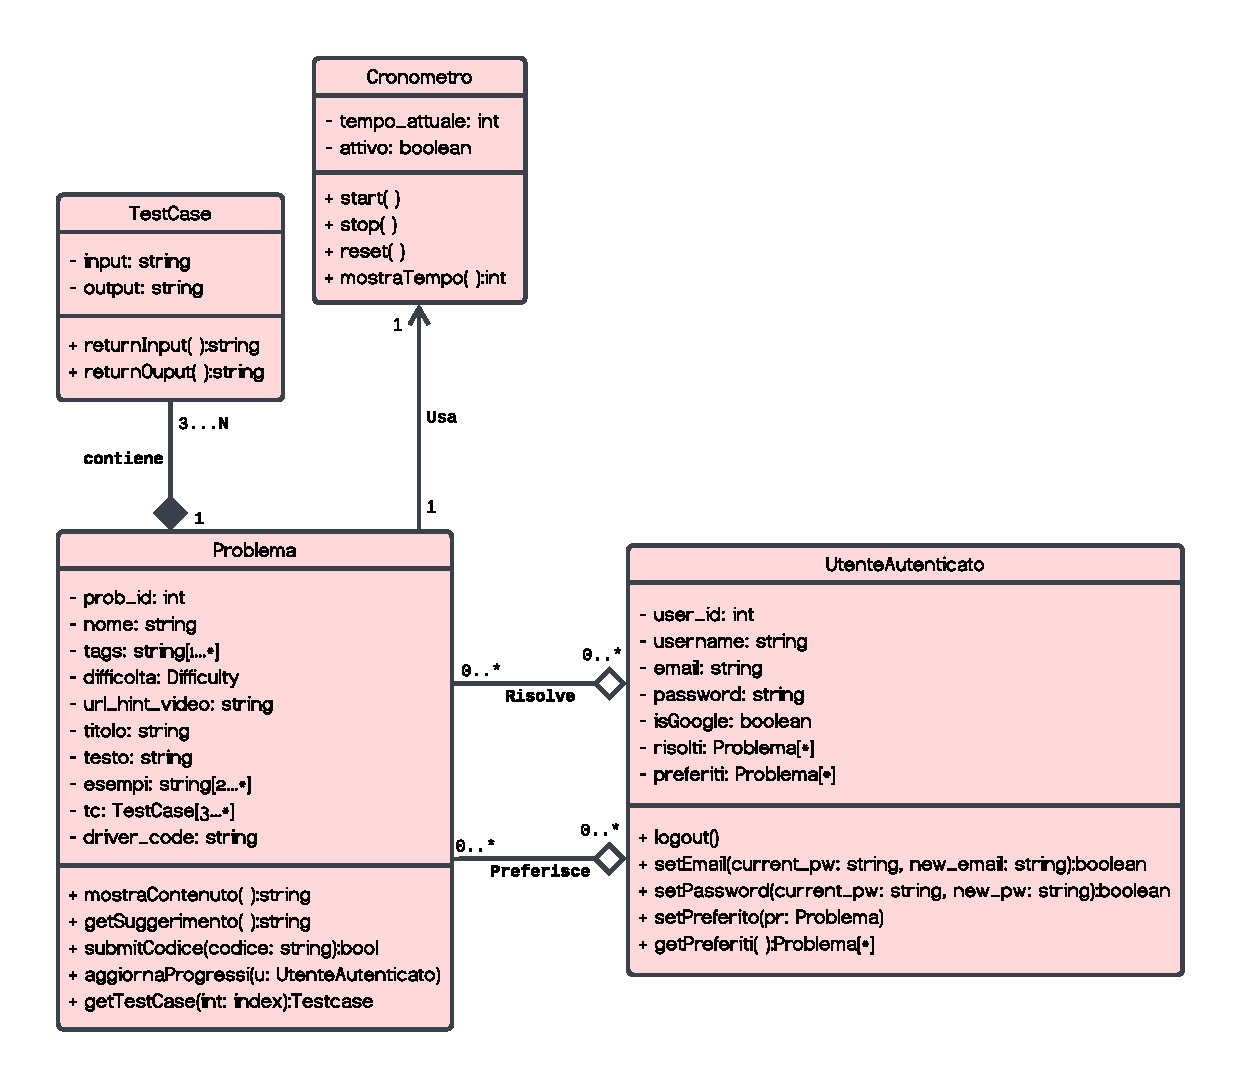
\includegraphics[scale = 0.85]{materiale/class-esercitazione.pdf}
\caption{Classi dedotte dal componente \textit{Pagina di esercitazione}}
\label{esercitaz}
\end{figure}

\noindent La classe \texttt{Problema} è definita come segue:
\begin{itemize}
    \item \texttt{nome}, \texttt{tags}, \texttt{difficolta}, \texttt{url\_hint\_video}:
    questi rappresentano i campi descrittivi del problema, come specificati nel
    documento D1. La difficoltà può assumere solamente uno dei valori
    definiti dal dominio del tipo enumerato \texttt{Difficulty}.

    \item \texttt{titolo}, \texttt{testo}, \texttt{esempi}: i dati strutturali del problema.

    \item \texttt{tests}: i test cases utilizzati per verificare il codice
    sottoposto dall'utente.

    \item \texttt{driver\_code}: il frammento di codice predefinito che
    viene mostrato nella zona di inserimento del codice, nell'area di
    esercitazione.

    \item \texttt{preferito:} contatore che registra la quantità di utenti
    registrati che hanno contrassegnato questo specifico problema.

    \item \texttt{mostraContenuto}: questo metodo permette di comporre
    l'area di consultazione del problema, con il suo titolo, testo ed
    esempi.

    \item \texttt{getSuggerimento}: questo metodo rende disponibile
    all'esterno l'indirizzo del video YouTube associato (il suggerimento),
    in particolare per permettere al catalogo di riprodurlo.

    \item \texttt{submitCodice}: il codice scritto dall'utente viene
    sottoposto ai test.

    \item \texttt{aggiornaProgressi}: questo metodo viene utilizzato
    quando un utente autenticato risolve il problema con successo.

    \item \texttt{getTestCase}: i test cases associati al problema
    vengono forniti esternamente per mostrarli nell'area di esercitazione.

\end{itemize}
Ogni problema memorizzato nel database viene identificato grazie a
\texttt{prob\_id}.
\\\\
Al fine di alleggerire la classe \texttt{Problema}, è stata accolta la scelta di
dedicare una classe \texttt{TestCase}. Essa ha il compito di raccogliere le informazioni
chiave necessarie al test del codice fornito dall'utente (il quale si esercita
sul problema specifico): \texttt{input}, \texttt{output} e dei metodi che rendono
questi attributi disponibili all'esterno.
Si noti che la relazione che unisce \texttt{TestCase} e \texttt{Problema} è
una \textbf{composizione} (indicato dall'estremità romboidale nera): i testcases
sono infatti associati a specifici problemi, come espresso dalle cardinalità,
ma non hanno alcun significato se il problema specifico al quale dovrebbero
essere associati non esiste.

Altra parte integrante della Pagina di Esercitazione è la classe \texttt{Cronometro},
che prevede le semplici funzionalità per mostrare il tempo registrato in secondi,
essere avviato, fermato e reimpostato a 0 (condizioni più dettagliate
di questa classe sono mostrate nel codice OCL delle prossime sezioni).


\newpage
\subsection{Gestione profilo: preferiti e progressi}
Il componente \textit{Gestore Profilo}, descritto nel diagramma dei componenti
del documento D1, è costituito dalla classe \texttt{UtenteAutenticato},
come anticipato nelle sezioni precedenti. In Figura \ref{profile} sono
mostrate le associazioni che mettono in relazione la classe \texttt{UtenteAutenticato}
e la classe \texttt{Problema}, al fine di descrivere le seguenti
caratteristiche:
\begin{itemize}
    \item Risolve: questa relazione di aggregazione evidenzia la possibilità
    per un utente autenticato di memorizzare (automaticamente) i problemi
    risolti con successo, definendo i progressi.

    \item Preferisce: con questa relazione di aggregazione, le classi
    \texttt{Problema} e \texttt{UtenteAutenticato} vengono unite per realizzare i preferiti
    dell'utente.
\end{itemize}

\begin{figure}[H]
\hspace*{-2.7cm}
\centering
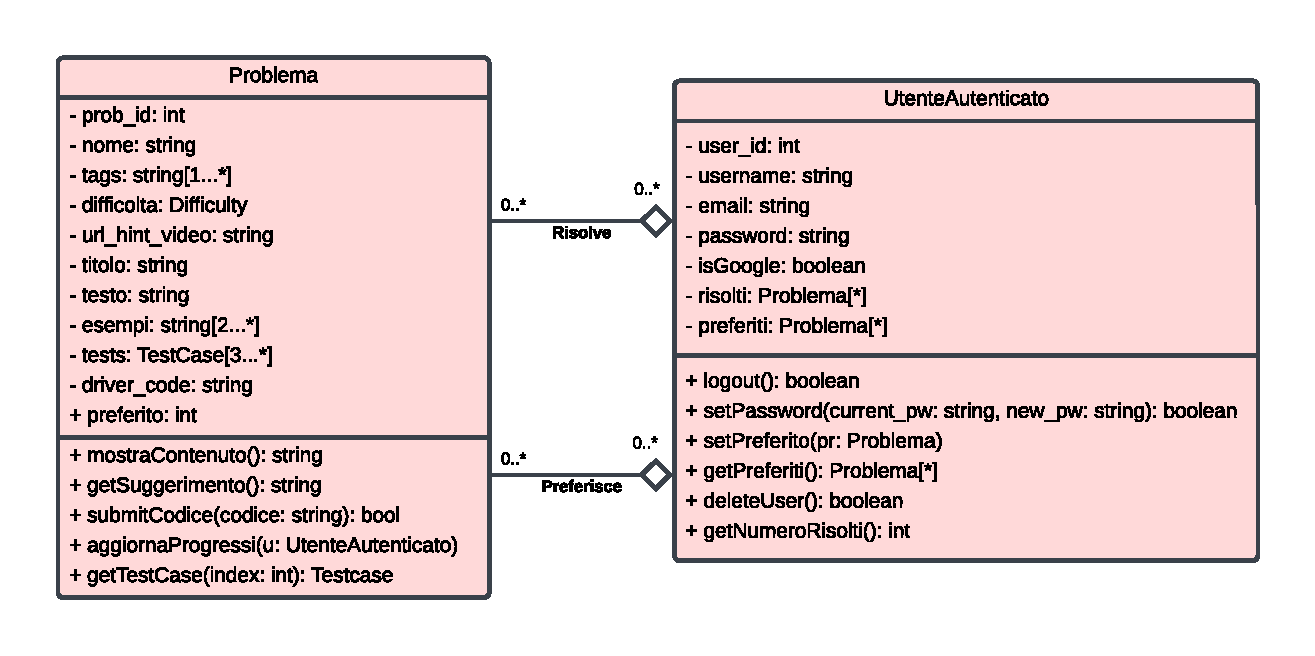
\includegraphics[scale = 0.8]{materiale/class-profilo.pdf}
\caption{Associazioni tra \texttt{Problema} e \texttt{UtenteAutenticato}}
\label{profile}
\end{figure}




\newpage
\section{Specifiche in codice OCL}
Nella sezione che segue viene descritta formalmente la logica prevista
nel comportamento di alcune classi, in relazione alle loro operazioni
possibili. Il codice OCL impiegato consente di esprimere tale logica,
non descrivibile con i soli diagrammi delle classi in UML.


\subsection{Autenticazione}
\begin{figure}[H]
\centering
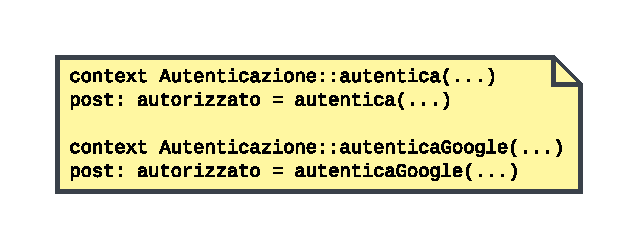
\includegraphics[scale = 0.9]{materiale/ocl-autenticazione.pdf}
\end{figure}

\subsection{Recupero della password}
Con riferimento alla classe \texttt{RecuperoPwUtente},
l'attributo \texttt{email} deve essere sempre presente affinché la classe
possa essere impiegata.
\begin{figure}[H]
\centering
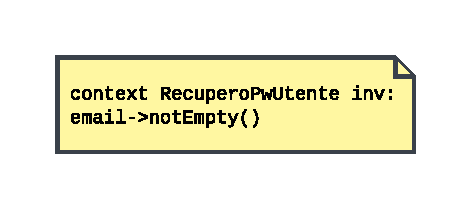
\includegraphics[scale = 1]{materiale/ocl-recuperoemail.pdf}
\end{figure}
%\noindent Inoltre, \texttt{cambiaPassword}, può essere utilizzato per il
%recupero di account non-Google e solo se viene fornita una password
%valida da associare ad un account esistente (da recuperare) con indirizzo
%email specificato.
%\begin{figure}[H]
%\centering
%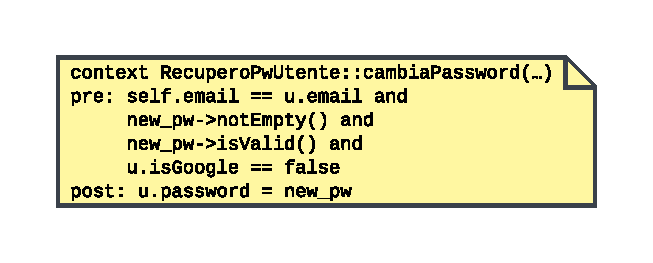
\includegraphics[scale = 0.9]{materiale/ocl-recuperopassword.pdf}
%\end{figure}

\subsection{Utente autenticato}
La classe \texttt{UtenteAutenticato} prevede che i campi \texttt{user\_id},
\texttt{username} e \texttt{email} non siano mai vuoti, affinché un
account (anche se creato con Google-SignIn) possa essere ufficialmente registrato
sulla piattaforma.

\begin{figure}[H]
\centering
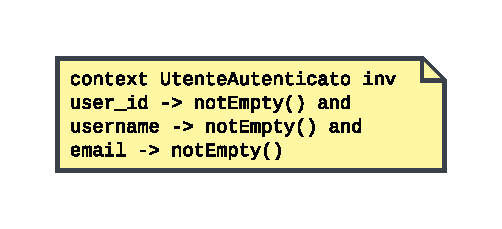
\includegraphics[scale = 0.9]{materiale/ocl-utenteautenticato.pdf}
\end{figure}

\subsection{Modifica della password}
Gli utenti registrati con account Google non possono creare una nuova
password, non avendo la necessità di utilizzare quel tipo di dato.
La password dell'account può essere modificata qualora la password
attuale venga inserita correttamente e solo se la nuova password
è valida (\textbf{RNF 11} - Password sicura).

\begin{figure}[H]
\centering
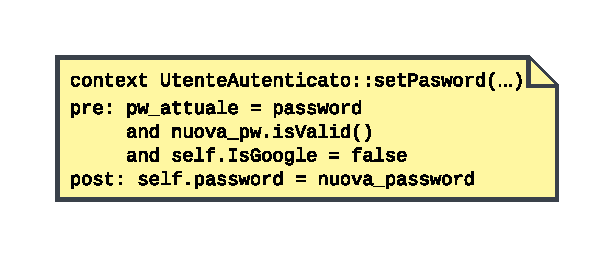
\includegraphics[scale = 1.1]{materiale/ocl-newpassword.pdf}
\end{figure}

\subsection{Modifica del catalogo}
Nei documenti precedenti viene sottolineato che i campi descrittivi e
strutturali di ogni problema del catalogo devono essere sempre presenti.
Con riferimento alla classe \texttt{UtenteAmministratore}, oltre alle
cardinalità specificate tra parentesi quadre per alcuni parametri in input
dei metodi di tale classe, vengono
definite queste ulteriori condizioni:
\begin{figure}[H]
\centering
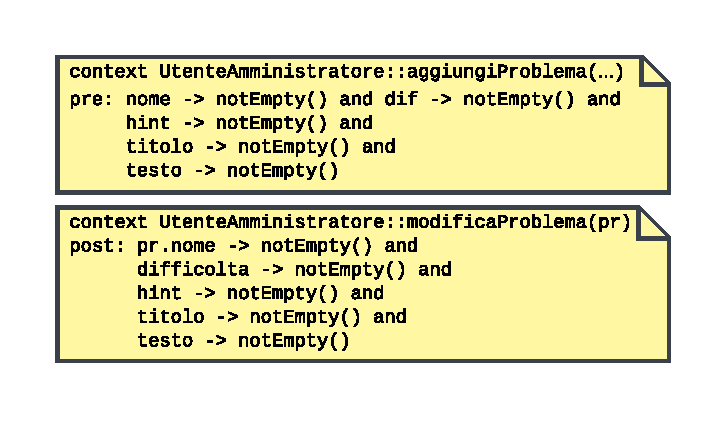
\includegraphics[scale = 1]{materiale/ocl-amministratore.pdf}
\end{figure}

\subsection{Problema}
Ogni problema potrebbe avere un numero diverso di test case (sempre e
comunque maggiore o uguale a 3). Viene dunque posto il seguente vincolo
sulla selezione dei test case disponibili per ogni problema nel catalogo,
facendo riferimento alla classe \texttt{Problema}:
\begin{figure}[H]
\centering
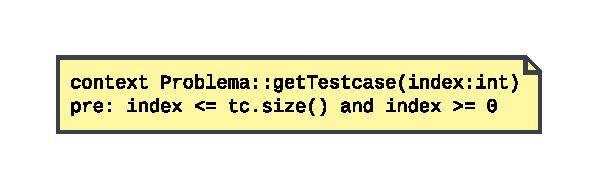
\includegraphics[scale = 1.1]{materiale/ocl-problemaindicetc.pdf}
\end{figure}

\noindent Tenendo sempre in considerazione la classe \texttt{Problema}, è
previsto che il valore di \textit{preferito} sia sempre non negativo:
\begin{figure}[H]
\centering
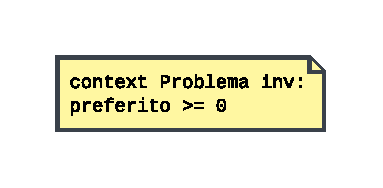
\includegraphics[scale = 1.1]{materiale/ocl-problemainv.pdf}
\end{figure}

\subsection{Test Cases}
La classe \texttt{TestCase} prevede che i suoi attributi non siano mai
vuoti, affinché i test cases possano essere utilizzati per verificare
la correttezza del codice sottoposto dall'utente.

\begin{figure}[H]
\centering
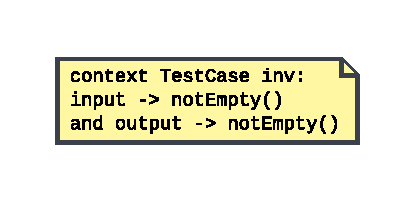
\includegraphics[scale = 1.1]{materiale/ocl-testcase.pdf}
\end{figure}

\newpage
\subsection{Cronometro}
Sono elencati di seguito i dettagli riguardanti il funzionamento della
classe \texttt{Cronometro}:
\begin{itemize}
    \item Il \texttt{tempo\_attuale} registrato può assumere solamente
    valori positivi.

    \begin{figure}[H]
    \centering
    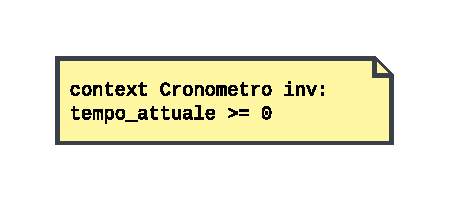
\includegraphics[scale = 1]{materiale/ocl-tempo.pdf}
    \end{figure}

    \item Il metodo \texttt{start} esegue l'avvio della registrazione
    del tempo trascorso, a partire dal valore contenuto in
    \texttt{tempo\_attuale}, nella situazione in cui il cronometro non è
    attivo. L'attributo \texttt{attivo} viene opportunamente aggiornato.
    L'operazione opposta è rappresentata da \texttt{stop}, utilizzabile
    quando il cronometro è attivo. Il
    metodo \texttt{reset} riporta il cronometro al suo stato iniziale,
    quindi inattivo e tempo registrato 0.

    \begin{figure}[H]
    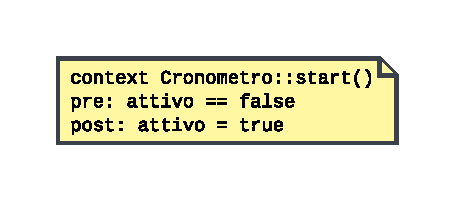
\includegraphics[scale = 0.9]{materiale/ocl-start.pdf}
    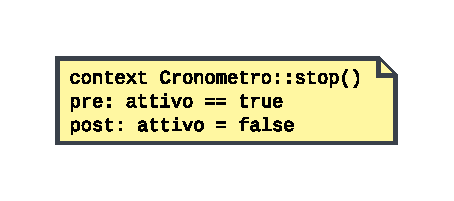
\includegraphics[scale = 0.9]{materiale/ocl-stop.pdf}
    \centering
    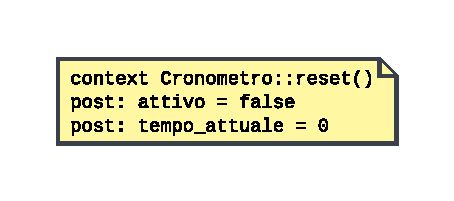
\includegraphics[scale = 0.9]{materiale/ocl-reset.pdf}
    \end{figure}
\end{itemize}









\newpage
\section{Diagramma delle classi con codice OCL}
La Figura \ref{umlocl} unisce le classi e le specifiche in OCL precedentemente definite.

\begin{figure}[H]
\centering
\hspace*{-2.5cm}
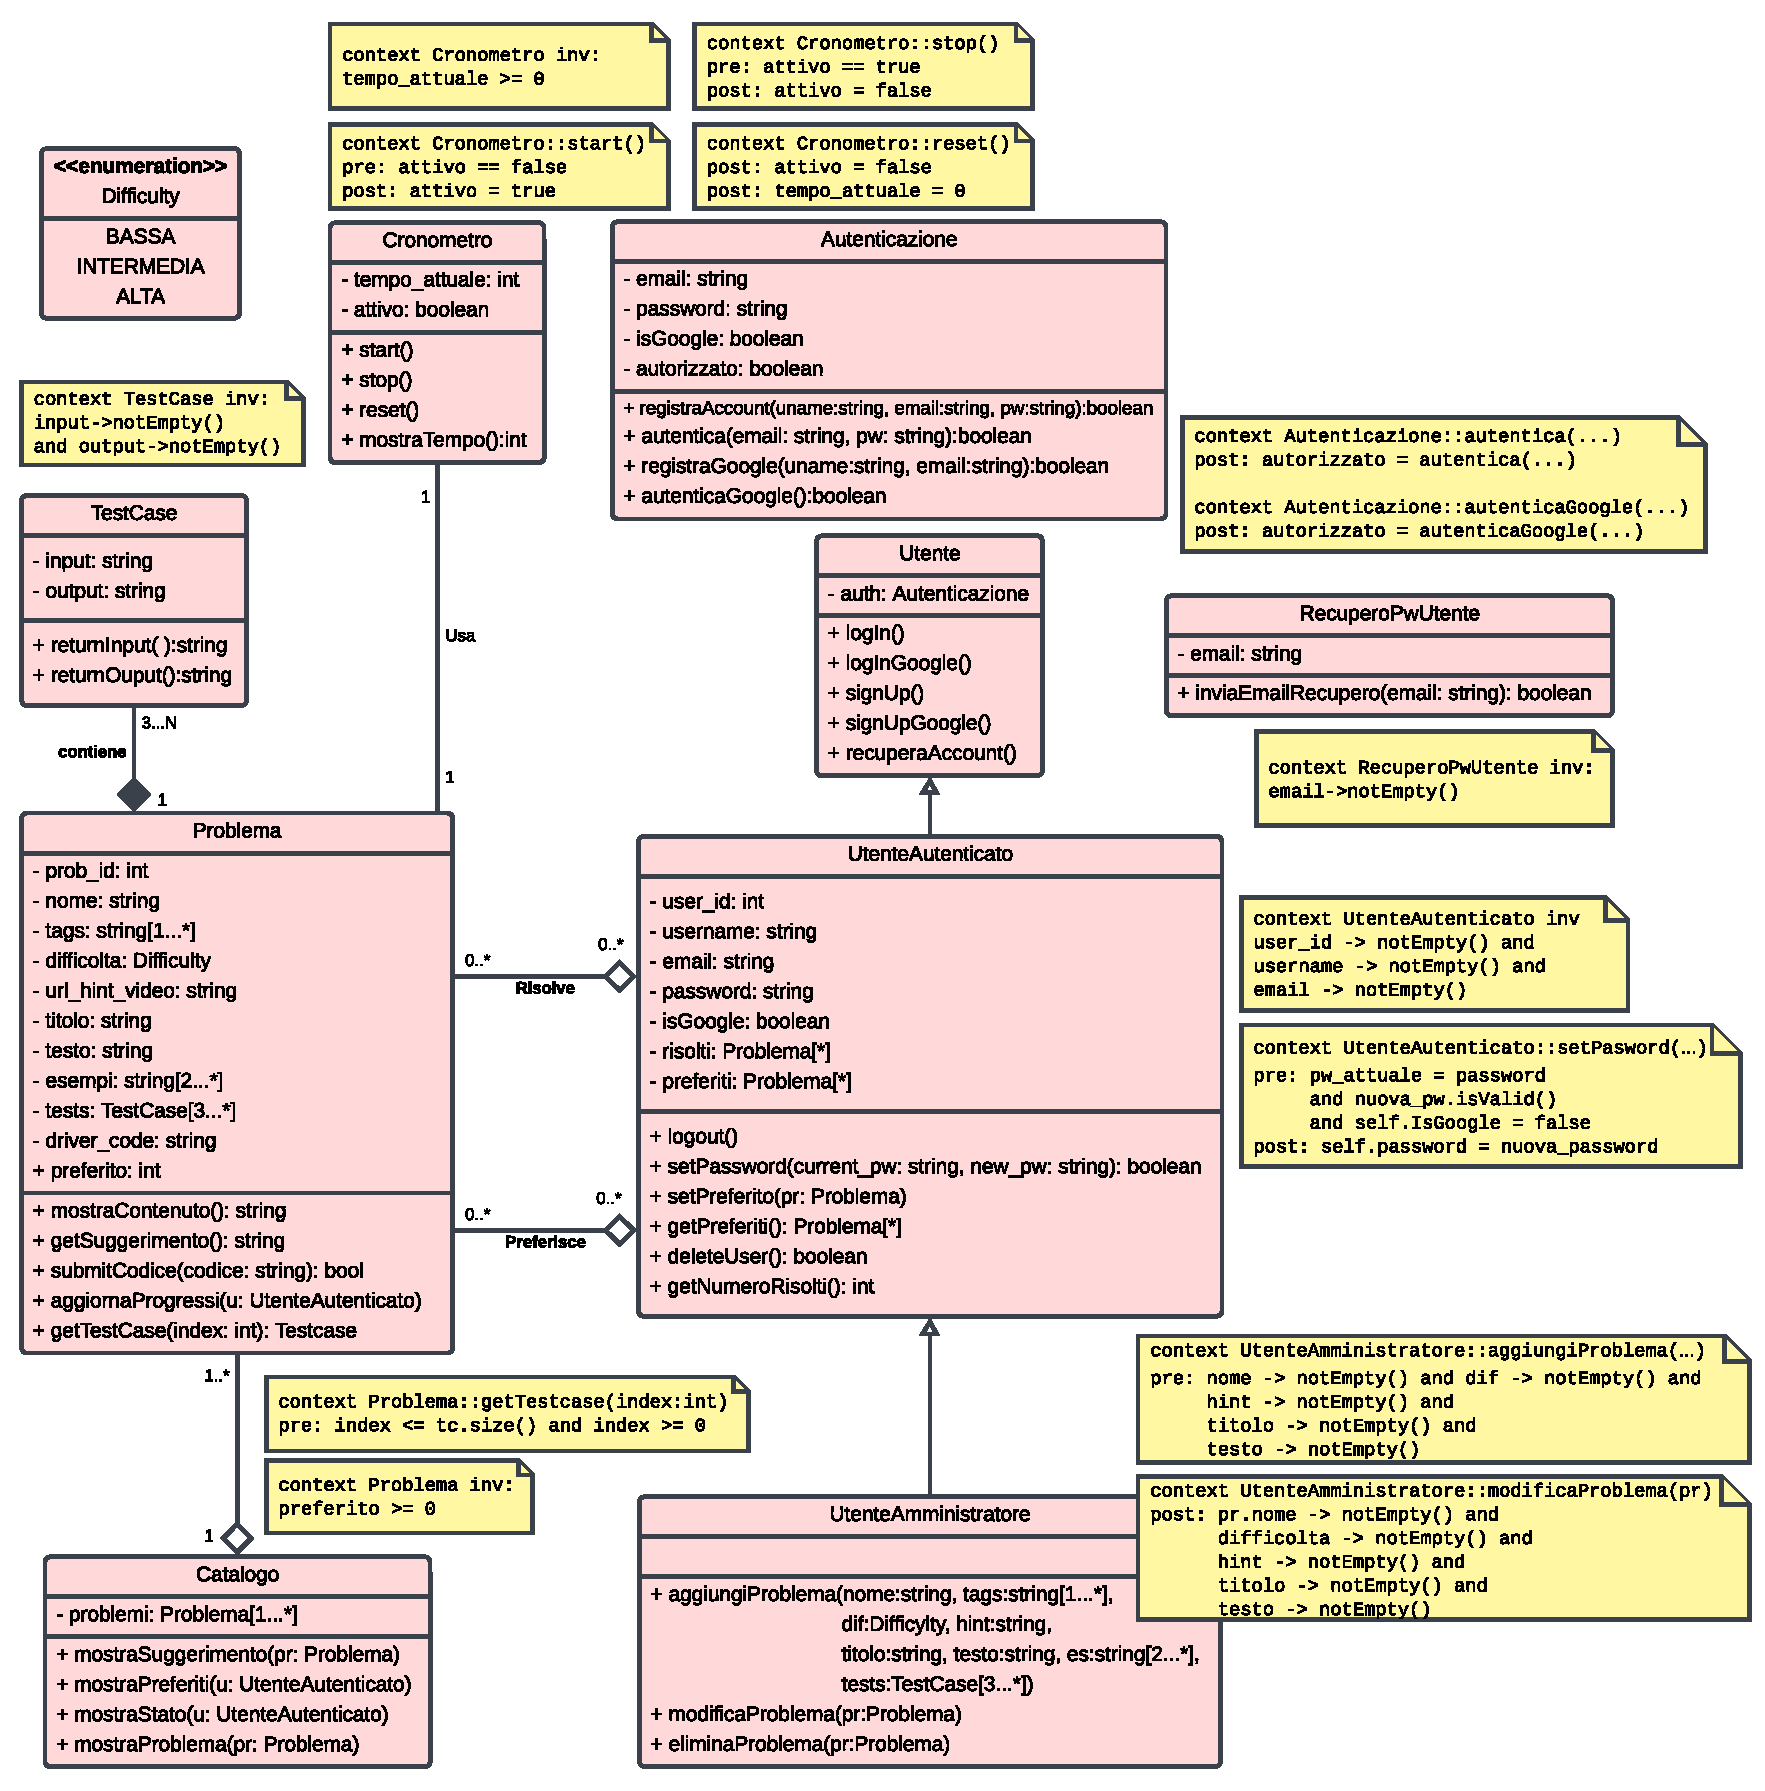
\includegraphics[scale = 0.6]{materiale/classdiagram.pdf}
\caption{Diagramma delle classi insieme al codice OCL}
\label{umlocl}
\end{figure}

\end{document}